\chapter{Literature Review \& Goals} % 4 pages


    In this chapter, we are going to give an overview of the information that was acquired about recommender systems during the project and also include some explanations for things brought up in the design of the project. At the end of this chapter, we are going to explain the goals of the project before we describe the design for the recommender.

    \section{Information Filtering Systems}

        An information filtering system is a system that removes unwanted information. Nowadays there is so much media being created every day it can be very difficult to keep on top of everything coming out so it is very easy to miss movies you might be interested in. Recommender systems are a subset of Information Filtering systems.  A recommender system aims to predict the rating a user would give something based on some information it has. A recommender system aims to cut through all the extra data that exists now and bring you the most important information. Examples are the Netflix recommender that gives you an infinite list of movies you watch or Amazon's similar items recommender that gives you items other people like you, buy based on your purchase history. Major recommender systems can use either Collaborative filtering or Content-based filtering to create recommendations. 


    \section{Collaborative Filtering}
        Collaborative Filtering uses user behavior to link people together. This system does not use information or metadata about what you are recommending to make a recommendation. An example of this is the way \textit{Last.fm} recommends music to its users. It creates a station that plays music that people similar to you have played that you have not. They determine how similar you are to another user based on the common music tracks that you both listen to regularly. This has advantages that similar people are likely to listen to the same music so recommendations can be quite good. This type of recommender can be constrained by the cold start problem wherein the case of Last.fm the system needs to be seeded with a large amount of a users' music to be good at recommending. In this system, user taste can be acquired in different ways. It can be collected either implicitly or explicitly. You can collect data explicitly by asking users to rate pieces of data or using search results to form data points. You can also use information from other sources such as social media or their internet search results as implicitly collected data.


    \section{Content-Based Recommender}
        Another option for building a recommender system is to use content-based filtering. This is done using the information about what you are recommending instead of the users in the system. An example of this would be recommending music based on its metadata such as artist or the beats per minute of the song. If a user listens to songs that have a common bpm regularly it would make sense to recommend them more songs with that same bpm. This does not require as much seed data which means the cold start problem affects it less. The recommendations can be made more accurate the more information the system has. It can create more interesting connections between what a user has listened to and what they have not. 


    \section{Recommender System Problems}\label{sec:RecommenderSystemProblems}
        As we have mentioned above there are some problems that can be associated with certain types of recommenders. Collaborative filtering has problems such as the cold start problem and problems related to scalability and sparsity. Recommenders can have problems that are not created by the type of filtering they use.  

        \subsection{Cold Start Problem}
            When a new user signs up to a movie recommender that uses collaborative filtering it will be unable to create recommendations because it has no information about the user. As movies are added it will still be difficult to recommend anything until there is a significant amount of information that will allow the recommender to match you to other users that have similar viewing patterns. These types of recommenders need to be seeded with a set of ratings, to begin with in order to, recommend. This does not apply to recommenders that use Content-based matching as once you have one movie the system can start recommending based on that movie's metadata. This can be fixed by asking users to pull in information from other sources or by using a hybrid recommender that used multiple techniques. Movie lens \cite{10.1145/2827872} solves this problem by having users create a profile and then asking them to rate some movies as they create their profile so it is not empty.

        \subsection{Other problems}
            Scalability and Sparsity:
            As the size of a dataset increases the amount of computation necessary to calculate recommendations. Often recommending involves matrix calculations the size of the calculations increases the more examples and features involved. 
            If for example, the number of movies increases the matrices begin to get sparse meaning there will be lots of 0s in the dataset. This takes up space and does not help calculations. 


        \subsection{User Privacy}
            Recommenders are a fairly new invention. They were first mentioned in the year 1990 by Jussi Karlgren at Columbia University. He talked about them in relation to a "digital bookshelf". Nowadays most large websites that serve some form of content will have a recommender built-in. Google's search engine changes the results of the searches based on your history. YouTube will recommend videos based on a complex algorithm. Amazon has a recommender in the shopping website and integrated  into the streaming site Amazon prime video. Netflix and Spotify both have them. To create a recommender that can compete to today's standards involves collecting large amounts of data about all types of people to create good recommendations. Along with collecting large amounts of information comes the privacy concerns of what are these companies going to do with all this collected data. Some of these companies will go to great lengths to keep the algorithms as trade secrets. Once this data has been collected in can be used to create recommendations but also to swing elections. In the case of Cambridge Analytica who used data Facebook collected to target users with recommendations based on their data to swing their political views.
            
            As part of the growth of social media over the last 10 years, the recommendation of personalised content has grown with it. Part of the reason social media is so addictive is the endless scrolling through content that has been recommended to you. Websites like YouTube and Facebook keep you on their platform be trying their best to recommend a person content that will keep them there. In extreme cases, this can be detrimental to one's health as shown in \cite{SocialMediaAddiction}. As many recommender systems in these big websites are completely automated they often recommend any content that a user might like. This can lead to unsavory content being recommended to a user. Recommenders are supposed to just recommend the best content for a user so they are doing their jobs correctly. 
        
        

    \section{Correlation}\label{sec:pearsonCorrelation}
        As part of a collaborative-filtering recommender, correlation is often used to predict the relationship between users. Correlation is a statistical relationship between two variables. It can be used to predict relationships between data. It is a measure of the degree to which two variables are linearly related. For example, we can get the relationship between two people based on their movie ratings on a selected number of films. The most popular measure of the correlation between the two values is the Pearson Correlation Coefficient. It is defined as the quality of least-squares fitting to the original data, normalized to the square root of their variances. The Correlation Coefficient is just a measure of the correlation between the two values.  

        Correlations lie between -1 and 1. A value of -1 indicates that the two values are perfectly negatively linearly related. If the value is 0 this means there is no linear relation between the two variables although there might be a non-linear relation between the two values. There are examples of data and the produced Pearson Correlation shown in \ref{fig:PearsonCorrelationPic}

        \begin{figure}
            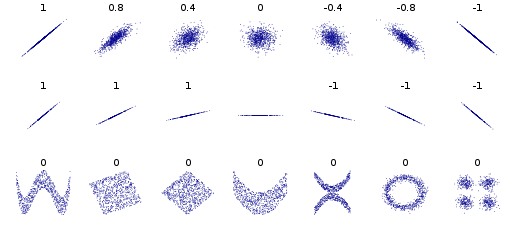
\includegraphics[width=125mm,scale=0.5]{PearsonCorrelation.png}
            \label{fig:PearsonCorrelationPic}
            \caption{Diagram showing various correlations Created by Denis Boigelot}
            \cite{PearsonCorrelationImage}
        \end{figure}

    

    \section{Explainable AI}
        In recent years there has been an effort to create explanations for recommendations that are created from artificial intelligence models. Explainable artificial intelligence is the section of AI that comes up with solutions to the problems relating to explaining the methods and techniques used in the application of AI technology. There are two types of models people use when creating artificial intelligence, white and black box models.  A model is a representation of a system that is created in order to understand the subject the model represents. In order to grow the trust that can be placed into models generated from artificial intelligence work has been done to increase their capacity to explain themselves. If they can explain themselves we are more likely to trust them. 

        \subsection{White Box Model}
            A white-box model is a model that is considered interpretable due to the simple structure. A small decision tree or sparse linear model are examples of this. Someone would be able to easily follow the selections down a small decision tree and it would be able to explain itself. A sparse linear model means many of the coefficients are 0. This leads to a model that is easy to understand as many of the features that are included in the prediction are not relevant. These often have a lower accuracy but have higher explainability. In figure \ref{fig:DecisionTreePic} we can see a decision tree. Starting at the top of the tree one can work their way down looking at the choice that was made at each stop helping to explain the decision. 


            \begin{figure}
                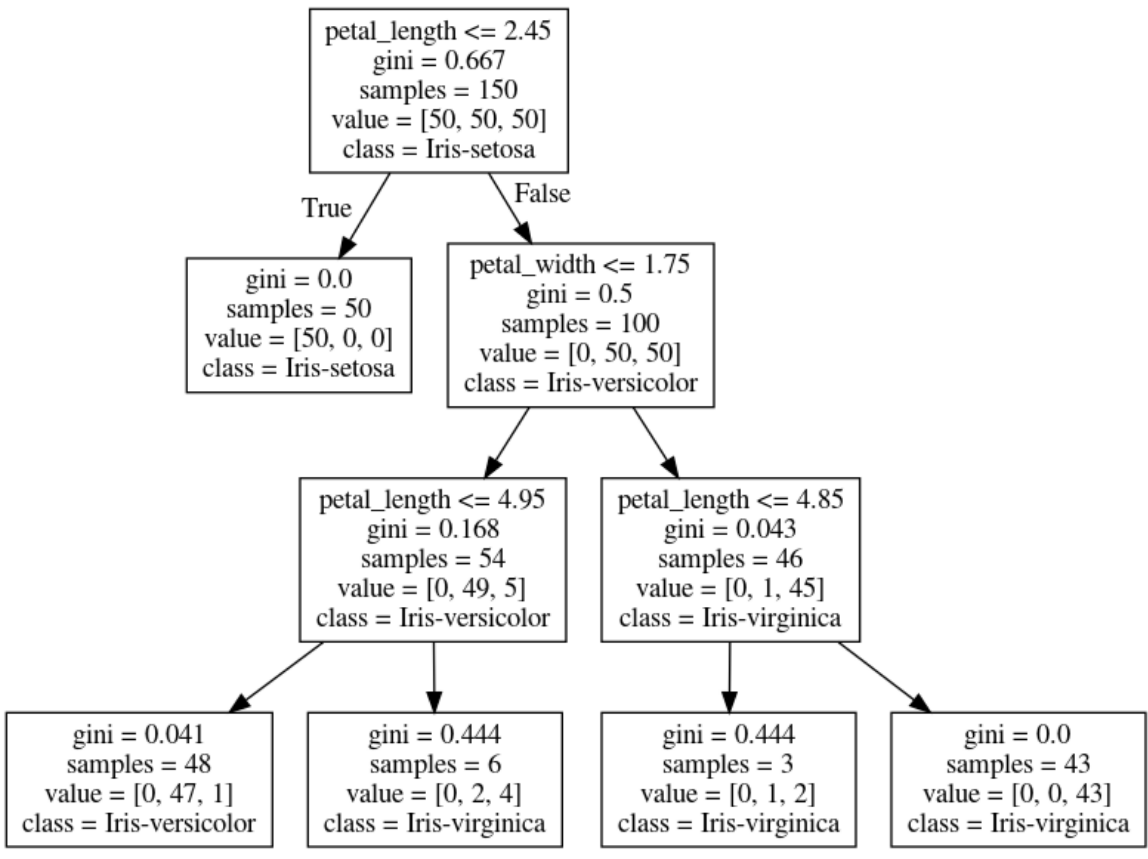
\includegraphics[width=125mm,scale=0.5]{DecisionTree.png}
                \label{fig:DecisionTreePic}
                \caption{Diagram showing a decision tree. Created by Derek Bridge  }
                \cite{DecisionTreeImage}
            \end{figure}


        \subsection{Black Box Model}
            A black box model on the other hand is a model where there is not an easy explanation that can be gathered. For example a neural network or ensembles such as Random Forests. A neural network is a system that is inspired by the neural networks in brains. These systems learn how to complete tasks based on examples given to them.
            Even big decision trees could be included in the black box model as it would be difficult for someone to discern an explanation from one as their size increases. Neural Nets are complicated enough that it would not be easy for a person to look through them and understand exactly how it came to its final decision using its weights. 


        \subsection{Explanation Methods}
            model-specific methods are methods of explanation that only work for a specific type of model. These can be made to work well for a single model but lack the ability to be general-purpose. Some methods only apply to decision trees for example LIME. LIME modifies the input data to a model and looks at the output in order to see what has changed. The output from LIME is a list of explanations that show the effect each feature of the input data had on the output. 

            Methods that work for any type of model are model agnostic. These are good because they are general purpose but often cannot  explain as well as model-specific methods as they have to work with more models.
            These have an advantage that they are much more flexible.
            There are many model-specific methods for explaining neural nets as they are popular and a type of black-box model.

        
    \section{Chain Based Recommenders}
        Another option for creating explanations for recommenders is the work done to create chain based recommendations \cite{Rana-Bridge-2017}. In this paper, they explored Recommendation by Explanation. In this system, they create a movie recommendation then get movies that are linked to that and create a chain. They then create explanations for the movies that are included in that chain. The Chain is created based on common keywords between the movies. This results in a high degree of serendipity, low population bias and high diversity. This is an interesting approach that seems to join a recommendation and an explanation. Conventionally these are considered separate tasks where recommendations are created and then explanations given.

    \section{Game-based Recommenders}
        \cite{10.1145/2792838.2799675}
        In this paper, they explore creating recommendations in a novel way. They have created a game with a purpose in order to solicit recommendations for movies.
        The game was hosted on Facebook so they could obtain information about the user likes their friends and what they like. This was then used to pick movies to include in the game. The player then has to pick the movies on the screen and assign them to a friend. This gets more difficult as the difficulty ramps up in the game. The answers from this could then be used to recommend a movie to a friend. They could then get the friends to rate the recommendations that were made satisfactory or not. Their results seemed to suggest this game was a better recommender than their collaborative filtering and content-based recommendation systems. 

    \section{Requirements}\label{sec:Requirements}
        in order to ensure the project matched what we planned we created a set of requirements both function and non functional that we could aim to complete.  
        \subsection{Functional Requirements:}
            \begin{itemize}

            \item The user must be able to search and rate movies to add to their profile.
            \item The user must be able to take part in user trials which accommodate a number of debates.
            \item The user should be able to view explanations for recommendations
            \item The user must be able to view the movies attached to their profile.
            \item The user must be able to view other users and the movies on their profile. 
            \end{itemize}
        \subsection{Non-Functional requirements}
            \begin{itemize}
                
            
            \item There must be a frontend for a user to interact with and there must be a single source where the data is stored. 
            \item The state of the user testing and the debates should be stored during operation.
            \item The user must be able to add their ratings to the system.
            \item The movies should create explanations for themselves. 
                \begin{itemize}
                    \item These may be scored relative to other explanations
                    \item Or they may be scored randomly for serendipity.
                \end{itemize}

            \item The system must be able to import information about new movies as they come out.
            \item The system should be able to compute the Pearson correlation between movies and users. 
            \end{itemize}